\section{Econometrics}
We used the following classical econometric methods on the \texttt{eec15} database:

\begin{itemize}
    \item Linear Regression
    \item Logistic Regression
    \item Probit Regression
\end{itemize}

For each of these methods, we used the same methodology: first, fit the model on \texttt{trim=1} data, then use the model to predict the probability that the \texttt{actop\_} variable is equal to 1 (i.e. that the observed person is \textit{unemployed}) for \texttt{trim=[2,3,4]} observations, and compare these results with the true values to assess the accuracy of the method.

Note that due to the close proximity of the logit and probit methods, we will only discuss the results of the logit model. We recommend any interested reader to go through the code and results of the probit method in the Appendix.

For the sake of clarity, for each model, we will first give the results, then provide an interpretation, focusing on the advantages and disadvantages of each method.

\subsection{Linear Regression}
As described in the \textit{Background} section, linear regression is arguably the simplest method we can use. The results of the regression can be found in Figure~\ref{fig:linear_regression_summary}.

\begin{figure}
    \centering
    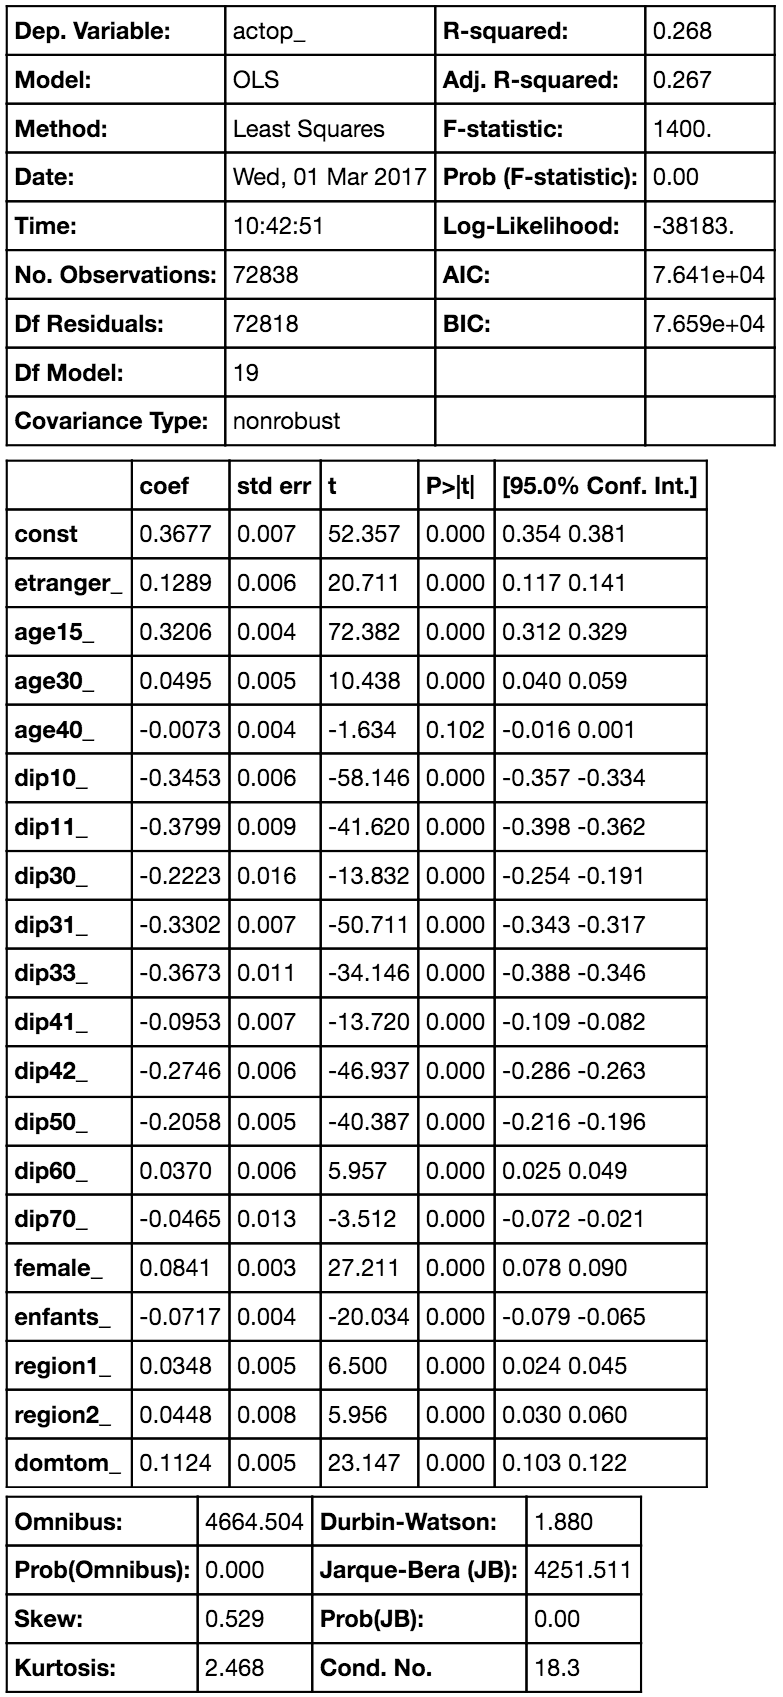
\includegraphics[scale=0.33]{img/linear_regression_summary}
    \caption{Linear Regression Summary}
    \label{fig:linear_regression_summary}
\end{figure}

Recall that when to classifying a binary variable, the result of a regression will be a \textit{probability of success}, which we can then use to conclude whether an individual is more or less likely to belong to one category or the other. The R-squared from this regression tells us that approximately 26\% of the explanation for an individual being active or not is explained by our set of independant variables. This number may seem low, but the regression is truly interesting if we look at the number/proportion of \textit{true positives} and \textit{true negatives} (or \textit{sensitivity} and \textit{specificity}):

\begin{center}
    \begin{tabular}{lcccc}
        \hline
                           & t1     & t2     & t3     & t4     \\
        \hline
        \texttt{actop\_=0} & 0.8805 & 0.8815 & 0.8802 & 0.8835 \\
        \texttt{actop\_=1} & 0.5455 & 0.5541 & 0.5322 & 0.5383 \\
    \end{tabular}
\end{center}

The method predicts people who are employed (\texttt{actop\_=0}) very well, getting the right result approximately 88\% of the time. In particular, since the proportion of employed is approximately 65\% in our database, a uniform guess would be correct 65\% of the time, so this method does in fact improve accuracy.

Also of note is the fact that all of our independent variables proved to be statistically signifiant, which is why we chose the same set of variables for all of our regressions.

\subsubsection{Marginal Effects}
We now turn to the information we were really looking for with this regression, namely \textit{how} our predictions are built and \textit{why} we obtain such results --- we thus look at marginal effects. As we have mentioned before, the linear regression model has the property that the coefficients of the regression are the marginal effects (with no further transformation needed).

We can see from the summary table (in Figure~\ref{fig:linear_regression_summary}) that the most important variables are \texttt{dip10\_}, \texttt{dip11\_}, \texttt{dip30\_}, \texttt{dip31\_} and \texttt{age15\_}. In other words, the level/degree of education, and age are important parameters in determining whether someone is unemployed or not.

Since all of our regressors are binary (dummy) variables, the marginal effect is the increase/decrease in probability of being unemployed (\texttt{actop\_=1}) relative to the reference group (no degree, more than 50 years old, male, French, living in a rural area in metropolitan France with no children).

\subsubsection{Limits}
The limits of the linear regression model are somewhat obvious: it is good if the relation between variables is (approximately) linear, but if the underlying relationship is of any other kind, the model will be inaccurate. Another limit, in our particular case, is that we \textit{may} obtain values superior $>1$ or $<0$, when we are in fact only dealing with binary values and hoping to get probabilities.

However, the main advantage that justifies the wide usage of linear regressions is the simplicity of interpretation. We can directly infer the causality relationships, compute statistical significance, and the R-squared to get an idea of how close we are to explaining the dependent variable. Another advantage is the simplicity of the computations, which makes this method both easy and fast to apply to large databases.


\subsection{Logistic Regression}
Logistic (or \textit{logit}) regression is slightly more complicated, but also better suited to our problem of determining a probability for a binary response variable. We ran the logit regression on the same set of regressors as for the linear regression, and the summary table can be found in Figure~\ref{fig:logit_regression_summary}.

\begin{figure}
    \centering
    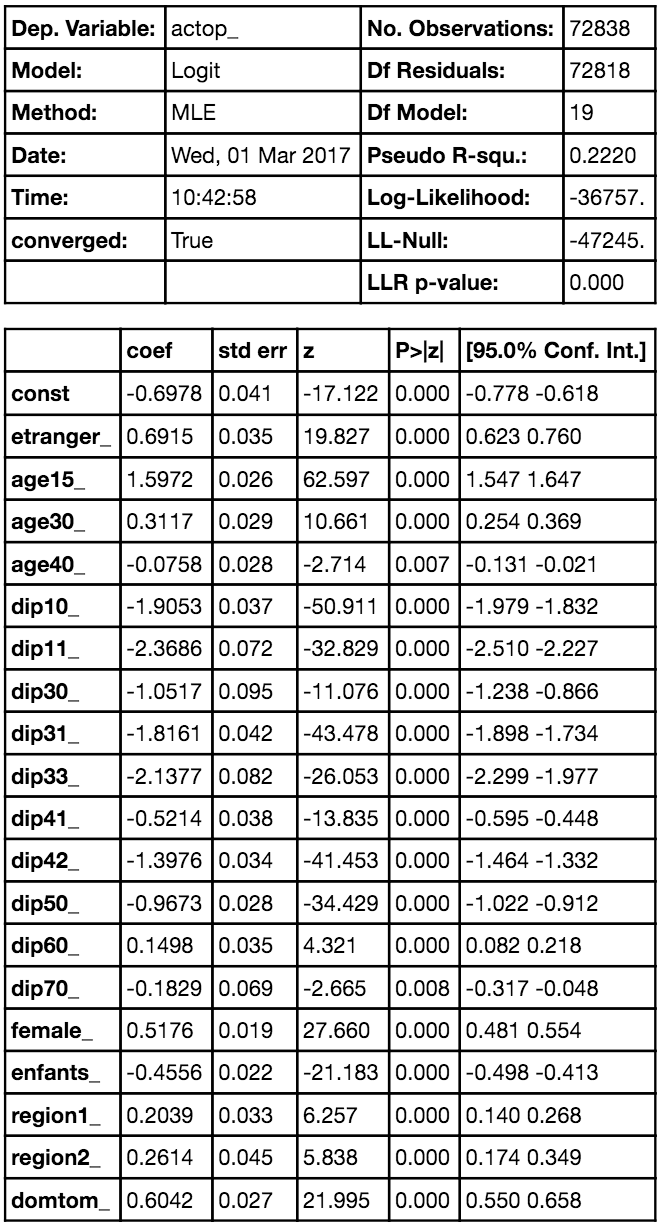
\includegraphics[scale=0.4]{img/logit_regression_summary}
    \caption{Logit Regression Summary}
    \label{fig:logit_regression_summary}
\end{figure}

Once again, we look at the accuracy of predicting $y=1$ for people that are actually unemployed, and $y=0$ for those that are employed.

\begin{center}
    \begin{tabular}{lcccc}
        \hline
                           & t1     & t2     & t3     & t4     \\
        \hline
        \texttt{actop\_=0} & 0.8729 & 0.8737 & 0.8723 & 0.8757 \\
        \texttt{actop\_=1} & 0.5591 & 0.5672 & 0.5459 & 0.5524 \\
    \end{tabular}
\end{center}

The prediction accuracy is very similar to what we get with a linear regression, in fact they are extremely close. Now, the question is how to interpret the results, and how to sense causality from this method.

\subsubsection{Marginal Effects}
While it is possible, mathematically, to derive the marginal effect of an independant variable (as we have seen in the \textit{Background} section), we only have discrete (binary) regressors in our specific case. Thus, while the derivative gives us a sense of the marginal effect, this effect may be different in reality.

In addition to this, the marginal effect of a variable is linked to the value of other independent variables, so we are focus on the mean marginal effects for each variable. More precisely, we look at the marginal effect of a given variable assuming that the other variables' are valued at their mean. The method (\texttt{brute\_force}) we use to calculate this empirically this is as follows:

\begin{enumerate}
    \item First, duplicate the original database and work on the new database
    \item Pick a regressor (e.g. \texttt{dip11\_}) and set it to 1 for all observations
    \item Find the probability of $y=1$ for all observations in both databases, using the model fitted to the original database.
    \item For each observation, take the difference in $P(y=1)$ between the two databases
    \item Take the mean of these differences
    \item Repeat this procedure for all regressors
\end{enumerate}

This method yields an empirical mean marginal effect for each of the independent variables.

Finally, we also wanted to get a sense of the accuracy of "rule-of-thumb" used to recover marginal effects from the coefficients of a logit regression (recall, this is $EM(x_1) \approx \frac{\beta_1^{logit}}{4}$. We find that this rule is not very accurate (the constant we divide by should be closer to $6$).

The values we obtained mathematically (and, up to a constant, through the "rule-of-thumb") are different from the empirical ones, which we explain by the non-continuity of the independent variable. However, for independent variables where we have enough data, the values are close, or differ in magnitude but not in sign, which gives us confidence as to the quality of our marginal effects (see Figure~\ref{fig:logit_marginal_effects}), and enables us to order the variables according to their importance and thus, to sense what determines the prediction we make.

% TODO(P2): what does Bastien mean by "Thus, even though using the derivative gives us a sense of the marginal effect, this effect may be different in reality."

\begin{figure}
    \centering
    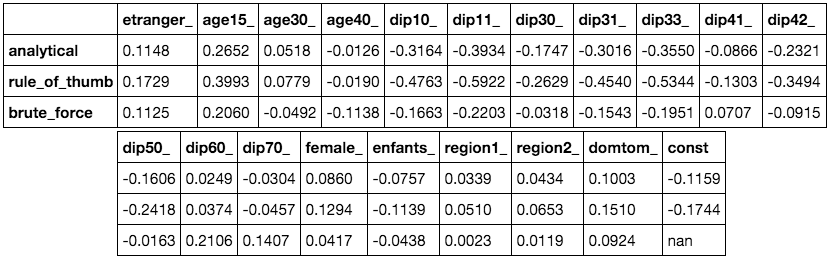
\includegraphics[scale=0.4]{img/logit_marginal_effects}
    \caption{Logit Marginal Effects}
    \label{fig:logit_marginal_effects}
\end{figure}

\subsubsection{Odds Ratios}
For the logit method, and in addition to the marginal effects, we also calculate the odds ratios to get an idea of the difference that having a given parameters or not makes on the response variable (see Figure~\ref{fig:logit_odds_ratios}). This will be interesting to compare with odds ratios from the Machine Learning algorithms. We use the following odds ratios formula:

\begin{equation}
    OR = \frac{P(y=1|x=1, X_{-1})/P(y=0|x=1, X_{-1})}{P(y=1|x=0, X_{-1})/P(y=0|x=0, X_{-1})}
\end{equation}

An odds ratio close to 1 means that the variable doesn’t add a lot of information. If it is close to zero, it means the variable strongly increases the probability that the individual works, and a ratio far beyond one indicates the opposite.

As a result we can conclude that being young makes it more likely that you are inactive, while having a higher degree of education makes it more likely that the person works.

\begin{figure}
    \centering
    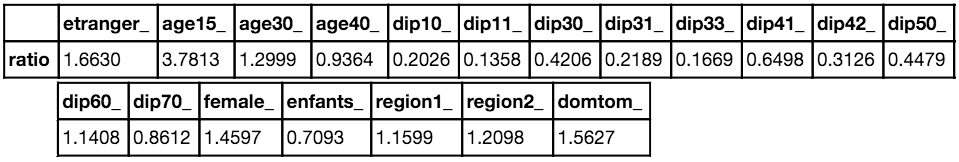
\includegraphics[scale=0.4]{img/logit_odds_ratios}
    \caption{Logit Odds Ratios}
    \label{fig:logit_odds_ratios}
\end{figure}

% TODO(P2): not sure what the next couple of paragraphs are about
% begin{attempt-at-rewriting}
% When looking at the shape of the curve of a logistic regression (see the \textit{Background} section), it is clear that marginal effects are biggest at the "mean individual" and get closer to zero for more "extreme" profiles.
% end{attempt-at-rewriting}

% According to the shape of the curve of a logistic regression, it is clear that the marginal effects are the biggest at the mean individual and get close to zero when you get extreme. So it even makes more sense to compare the marginal effects at the mean.

% All this makes it possible at a fairly low cost to get the marginal effects of the independent variables. It is by the way to be emphasized that with the logit method we can get the marginal effects of an independent variable at any point (any individual) and compute it analytically.
% This analytical computation is something we will lose with the Machine Learning algorithms.

\subsubsection{Limits}
The limits of logit exist by definition of the model. If the underlying relationship between variables is far from the logit curve, the model cannot predict accurately. In contrast, the model is significantly better than the linear model to predict binary/categorical variables --- its main advantage is the combination of fair accuracy and simplicity.

This makes it cheap to apply to large databases, while also providing results that are easy to interpet and explain, even to people with no background in statistics --- a great advantage that applies to regression models in general.
